% RESULTS CHAPTER
\chapter{Results}\label{ch:results}

In this chapter, the performance of the prediction model is analysed, and the discussion of the results are explored.
The machine learning algorithms are evaluated to determine the best model at predicting on unknown data.

\section{Performance Metrics}\label{sec:Performance Metrics}

The performance of any algorithm is evaluated by a few factors that are measured on the test dataset, where the trained model attempts to correctly predict the target field and this performance is then compared to its true outcome.
This assessment method is the norm on any binary classification problem and often will be visualised using a confusion matrix.
The confusion matrix is a simple visualisation in which the four possible permutations of predictions are displayed.
As seen in Figure~\ref{fig:ConfusionMatrix10}, it compares the number of predictions of wins and losses made by the model verses the number of real wins and losses found in the dataset. \\

\begin{figure}[h]
    \centering
    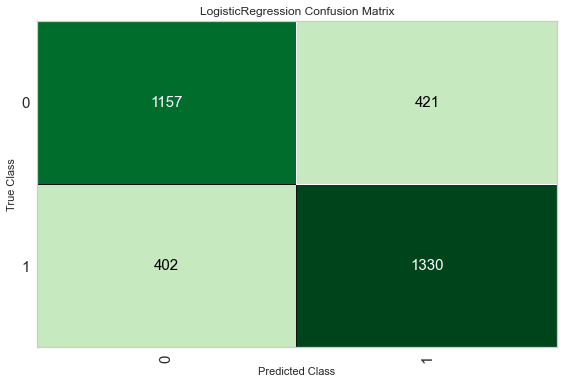
\includegraphics[width=0.8\textwidth]{figures/ConfusionMatrix10}
    \caption{A confusion matrix of a Logistic Regression Model trained on the 10 minute dataset}
    \label{fig:ConfusionMatrix10}
\end{figure}

On the y-axis the true class of the result can be seen, and on the x-axis there is the model's predicted class.
These four possible permutations are commonly referred to as follows:
\begin{itemize}
    \item \ac{TP} is seen in the bottom right of the matrix, this is when the predicted win actually reflects the true win.
    \item \ac{TN} is seen in the top left of the matrix, this is when the predicted loss actually reflects the true loss.
    \item \ac{FP} is seen in the top right of the matrix, this is when the predicted win is incorrect and the true class is a loss.
    \item \ac{FN} is seen in the bottom left of the matrix, this is when the predicted loss is incorrect and the true class is a win.
\end{itemize}

By collecting these outcome values, the effectiveness of each model is then able to be assessed via many performance metrics that are calculated using these values.
These measures each give an understanding of a model, with different implications depending on the objective of the project being assessed.
In this study, the focus is on assessing the correct classifications and there is little to no consequences for misclassification.
Therefore, the main criteria needed are the proportion of true classifications - aka the number of \ac{TP}s and \ac{TN}s compared to the whole prediction group.
This calculation is also known as the Accuracy of the prediction, and is calculated as follows:

\[ Accuracy = \frac{\sum TP + \sum TN}{\sum TP + \sum TN + \sum FP + \sum FN} \]

This is considered the key metric for this problem, as our dataset is pretty balanced so the other metrics such as Precision and Recall are not as important.
Here Accuracy can help decide how well a given model is predicting the correct outcomes of an esports League of Legends match.
The Accuracy of a model is only an effective metric if higher than the balance of the dataset, thus must be greater than 52.8\% to show any improvement over guessing the balance of the data.
Other metrics such as AUC, Precision, Recall are also calculated and evaluated, these metrics are calculated as such:

\begin{gather*}
    Precision = \frac{\sum TP}{\sum TP + \sum FP}\\
    Recall = \frac{\sum TP}{\sum TP + \sum FN}\\
    FPR = \frac{\sum FP}{\sum FP + \sum TN}\\
\end{gather*}

A \ac{ROC} curve is a graph that plots the Recall verses the \ac{FPR}, it plots these performance metrics between the bounds of zero and one.
\ac{AUC}, is a measure that understandably calculates the area under the \ac{ROC} curve which provides a measure of performance across all possible classification thresholds~\citep{aucGoogle}.
Essentially, \ac{AUC} is the probability that a model can distinguish between a positive and negative class - in this study it represents the ability to distinguish wins from losses.
Therefore, to conclusively accept a model as a feasible option, the Accuracy and AUC are the two core metrics that a model will have to score sufficiently on and will ultimately be the performance indicators to evaluate with. \\

\section{Model Results}\label{sec:Model Results}
\subsection{10 Minute Model}\label{subsec:10-minute-model}

As seen in Table~\ref{tab:ModelResults10}, most of the machine learning algorithms score quite similarly.
The four metrics of Accuracy, AUC, Recall and Precision all are within a 5\% range for every algorithm tested.
Here the best performing machine learning algorithm is the Logistic Regression model, scoring an accuracy of 75.06\% and an AUC of 82.30\%.
This is closely followed by the Linear Discriminant Analysis at an identical accuracy, but with an AUC of 82.28\%. \\

\begin{table}[h!]
    \centering
    \begin{tabular}{l c c c c }
        \toprule
        \textbf{Model} & \textbf{Accuracy} & \textbf{AUC} & \textbf{Recall} & \textbf{Precision} \\
        \midrule
        Logistic Regression & 0.7506 & 0.8230 & 0.7798 & 0.7574  \\
        Linear Discriminant Analysis & 0.7506 & 0.8228 & 0.7813 & 0.7566 \\
        Ada Boost Classifier & 0.7469 & 0.8181 & 0.7747 & 0.7546 \\
        Naive Bayes & 0.7458 & 0.8128 & 0.7613 & 0.7599 \\
        Gradient Boosting Classifier & 0.7458 & 0.8407 & 0.7759 & 0.7529 \\
        Quadratic Discriminant Analysis & 0.7456 & 0.8363 & 0.7601 & 0.7604 \\
        SVM - Linear Kernel & 0.7436 & 0.0000 & 0.7769 & 0.7492 \\
        Light Gradient Boosting Machine & 0.7357 & 0.8316 & 0.7630 & 0.7453 \\
        Random Forest Classifier & 0.7316 & 0.8230 & 0.7498 & 0.7462 \\
        Extra Trees Classifier & 0.7248 & 0.8116 & 0.7459 & 0.7385  \\
        K Neighbors Classifier & 0.7061 & 0.7794 & 0.7276 & 0.7212  \\
        Decision Tree Classifier & 0.6804 & 0.6794 & 0.6969 & 0.6998 \\
        \bottomrule
    \end{tabular}
    \caption{A table showing the model results for the 10 minute dataset}
    \label{tab:ModelResults10}
\end{table}

Interestingly enough the decision tree based algorithms that were commonly used in previous studies such as Random Forest, appear to perform slightly worse than algorithms such as Logistic Regression or Linear Discriminant Analysis.
These techniques are techniques based on linear regression analysis that opt to find a linear combination of features that cause separation in a problem.
These results then may indicate that the problem of match outcomes in League of Legends is linearly separable.
The model for the 10-minute mark was chosen to be built upon a logistic regression technique.
Firstly, the model is tested across the data split by the stratified k-fold cross-validation and tuned afterwards.
The resultant performance metrics can be seen in Table~\ref{tab:Kfold10}.

\begin{table}[h]
    \centering
    \begin{tabular}{lcccccc}
        \toprule
        \textbf{} & \textbf{Accuracy} & \textbf{AUC} & \textbf{Recall} & \textbf{Precision} \\
        \midrule
        Mean & 0.7516 & 0.8226 & 0.7618 & 0.7682 \\
        Std & 0.0150 & 0.0169 & 0.0285 & 0.0116 \\
        \bottomrule
    \end{tabular}
    \caption{A table showing the mean metrics after 10-fold cross-validation}
    \label{tab:Kfold10}
\end{table}

Table~\ref{tab:Kfold10} shows very similar results to the previous stated values, meaning that the model tuning had very little effect on improving the model's performance.
It also gives a standard deviation on the core metrics of under 2\%.
During the modelling, the feature importance of the features included in the dataset were calculated.
Figure~\ref{fig:FeatureImport10} shows the average relative importance of each feature when using the 10-minute dataset.
The top 10 features by feature importance are presented down the y-axis in decreasing order according to their relative importance values.
The most important features are those related to the player performance inside their lanes such as `csdiffat10', `deathsat10' and `KillParat10', with more objective team-based features having lower importance in predicting the resultant outcome of a given match.
At first this seems counter-intuitive, especially when given that teams must destroy towers in order to eventually win the game.
However, it is likely that at this stage of the game there is very low likelihood that teams can effectively destroy towers, so the focus should be on progressing their individual leads inside their lane.
These leads that they garner are reflected in the three features mentioned previously, and should translate into further advantages in more objective oriented features in a later game-state.

\begin{figure}[h]
    \centering
    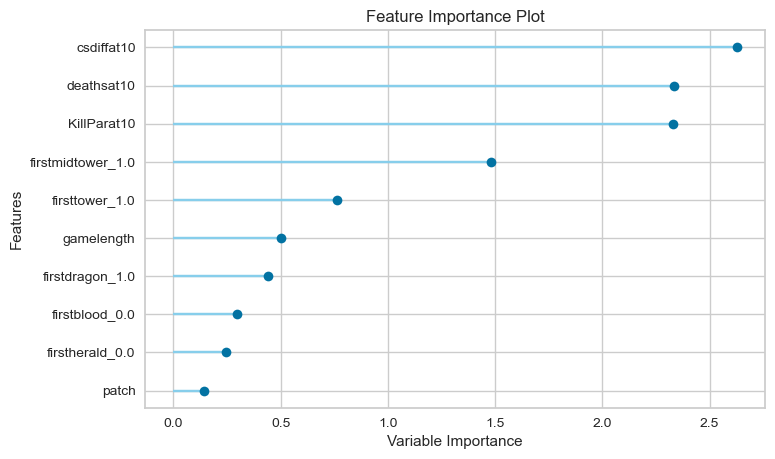
\includegraphics[width=\textwidth]{figures/FeatureImport10}
    \caption{A graph showing the imp 10 minute dataset}
    \label{fig:FeatureImport10}
\end{figure}




\subsection{15 Minute Model}\label{subsec:15-minute-model}

Table~\ref{tab:ModelResults15} highlights that once again that all the machine learning algorithms score within a 5\% range of the four key metrics tracked.
The two best performing machine learning algorithm remain the Logistic Regression model and the Linear Discriminant Analysis model, scoring an accuracy of 76.84\% and 76.87\%,  and AUC values of 84.74\% and 84.53\% respectively.

\begin{table}
    \centering
    \begin{tabular}{l c c c c }
        \toprule
        \textbf{Model} & \textbf{Accuracy} & \textbf{AUC} & \textbf{Recall} & \textbf{Precision} \\
        \midrule
        Linear Discriminant Analysis & 0.7687 & 0.8453 & 0.7994 & 0.7727 \\
        Logistic Regression & 0.7684 & 0.8474 & 0.7972 & 0.7733  \\
        Ridge Classifier & 0.7681 & 0.0000 & 0.7986 & 0.7721  \\
        Ada Boost Classifier & 0.7662 & 0.8418 & 0.7899 & 0.7741   \\
        Quadratic Discriminant Analysis & 0.7643 & 0.8578 & 0.7794 & 0.7772  \\
        Gradient Boosting Classifier & 0.7638 & 0.8601 & 0.7935 & 0.7690  \\
        Naive Bayes & 0.7589 & 0.8362 & 0.7694 & 0.7746  \\
        Light Gradient Boosting Machine & 0.7577 & 0.8551 & 0.7877 & 0.7635  \\
        SVM - Linear Kernel & 0.7562 & 0.0000 & 0.7835 & 0.7642 \\
        Random Forest Classifier & 0.7519 & 0.8483 & 0.7745 & 0.7623  \\
        Extra Trees Classifier & 0.7431 & 0.8359 & 0.7652 & 0.7545  \\
        K Neighbors Classifier & 0.7307 & 0.8067 & 0.7449 & 0.7470  \\
        Decision Tree Classifier & 0.6870 & 0.6854 & 0.7125 & 0.7021  \\
        \bottomrule
    \end{tabular}
    \caption{A table showing the model results for the 15 minute dataset}
    \label{tab:ModelResults15}
\end{table}




\subsection{20 Minute Model}\label{subsec:20-minute-model}

As seen in Table~\ref{tab:ModelResults20}, most of the machine learning algorithms score quite similarly.
The four metrics of Accuracy, AUC, Recall and Precision all are within a 5\% range for every algorithm tested.
Here the best performing machine learning algorithm is the Logistic Regression model, scoring an accuracy of 75.06\% and an AUC of 82.30\%.
This is closely followed by the Linear Discriminant Analysis at an identical accuracy, but with an AUC of 82.28\%.

\begin{table}
    \centering
    \begin{tabular}{l c c c c }
        \toprule
        \textbf{Model} & \textbf{Accuracy} & \textbf{AUC} & \textbf{Recall} & \textbf{Precision} \\
        \midrule
        Gradient Boosting Classifier & 0.8585 & 0.9433 & 0.8782 & 0.8586  \\
        Logistic Regression & 0.8583 & 0.9266 & 0.8648 & 0.8679 \\
        Linear Discriminant Analysis & 0.8583 & 0.9257 & 0.8513 & 0.8780 \\
        Quadratic Discriminant Analysis & 0.8582 & 0.9406 & 0.8706 & 0.8634 \\
        Ridge Classifier & 0.8581 & 0.0000 & 0.8511 & 0.8778 \\
        Ada Boost Classifier & 0.8559 & 0.9245 & 0.8623 & 0.8655 \\
        Random Forest Classifier & 0.8525 & 0.9387 & 0.8653 & 0.8581 \\
        SVM - Linear Kernel & 0.8521 & 0.0000 & 0.8504 & 0.8701 \\
        Light Gradient Boosting Machine & 0.8494 & 0.9392 & 0.8645 & 0.8538  \\
        Extra Trees Classifier & 0.8451 & 0.9315 & 0.8584 & 0.8512 \\
        K Neighbors Classifier & 0.8367 & 0.9057 & 0.8433 & 0.8482 \\
        Naive Bayes & 0.8284 & 0.9122 & 0.8509 & 0.8300 \\
        Decision Tree Classifier & 0.8024 & 0.8017 & 0.8140 & 0.8137\\
        \bottomrule
    \end{tabular}
    \caption{A table showing the model results for the 20 minute dataset}
    \label{tab:ModelResults20}
\end{table}


